\documentclass[11pt, a4paper]{article}
\usepackage{graphicx}
\usepackage{amsmath}
\usepackage{listings}
\usepackage{mathrsfs}
\usepackage{amssymb}



\title{Assignment 10} % Title

\author{Om Shri Prasath (EE17B113)} % Author name

\date{\today} % Date for the report
\begin{document}	

\maketitle % Insert the title, author and date
\section{Introduction}\label{introduction}

\begin{itemize}
  \item We are going to use DFT to implement convolution of two digital signals. One of the main use of DFT is to convolute digital input signal with a filter, since it is the fastest and most efficient way of doing so.
  \item Inverse DFT of multiplication of the DFT of two signals will give us what is known as the \textsl{circular convolution} of both the signals, which is defined as follows:
  \begin{center} If
  \begin{equation}
    Y(m) = X(m)H(m)
  \end{equation}
  then
  \begin{equation}
    y[n] = \sum_{m=0}^{N-1}x[(n-m)\%N]h[m]
  \end{equation}
  i.e.
  \begin{equation}
    y[n] = x[n]\circledast h[m]
  \end{equation}
\end{center}
  \item Normally, we would like to find only the linear convolution, which is the more useful convolution of the both, but finding circular convolution is easier, thus we find linear convolution from circular convolution using the following algorithm:
  \begin{itemize}
    \item First, we spilt the input signal into different parts, let the length of each part be L
    \item Let the length of filter signal be P. Thus, pad both the signals with zero, such that length of both the signals is N = L+P-1
    \item Now, do circular convolution for each section of input digital signal with the filter. We will get sections of y with N length
    \item The last P-1 samples of a y section will overlap with the first P-1 samples of the next y section. Thus, by adding the sections of y appropriately, we get the final output
  \end{itemize}
  \item Next, we analyze circular correlation, by using the example of Zadoff-Chu sequence. The Zadoff-Chu sequence have very interesting properties which will be demonstrated here.
\end{itemize}

\section{Python Code}
\subsection{Question 1}
\begin{itemize}
  \item Import the given filter and analyze it using the scipy.signal.freqz function.
\end{itemize}


\textit{\textbf{Code:}}

\begin{lstlisting}
import scipy.signal as sp
import numpy as np
import matplotlib.pyplot as plt
import pandas as pd
import time 

fil = pd.read_csv("/home/omshripc/Sem 4/EE2703/Answers/h.csv",
                  header=None)
fil = fil.values
fil = fil[:, 0]
w, h = sp.freqz(fil)

plt.title("Magnitude Response of Filter")
plt.plot(w, np.abs(h))

plt.ylabel(r"$|H(j\omega)| \to$")
plt.xlabel(r"$w \to$")

plt.show()

ph = np.unwrap(np.angle(h))
plt.title("Phase Response of Filter")
plt.plot(w, ph)

plt.ylabel(r"$\angle H(j\omega) \to$")
plt.xlabel(r"$w \to$")
plt.show()

\end{lstlisting}

\newpage
\begin{figure}[!tbh]
  \centering
  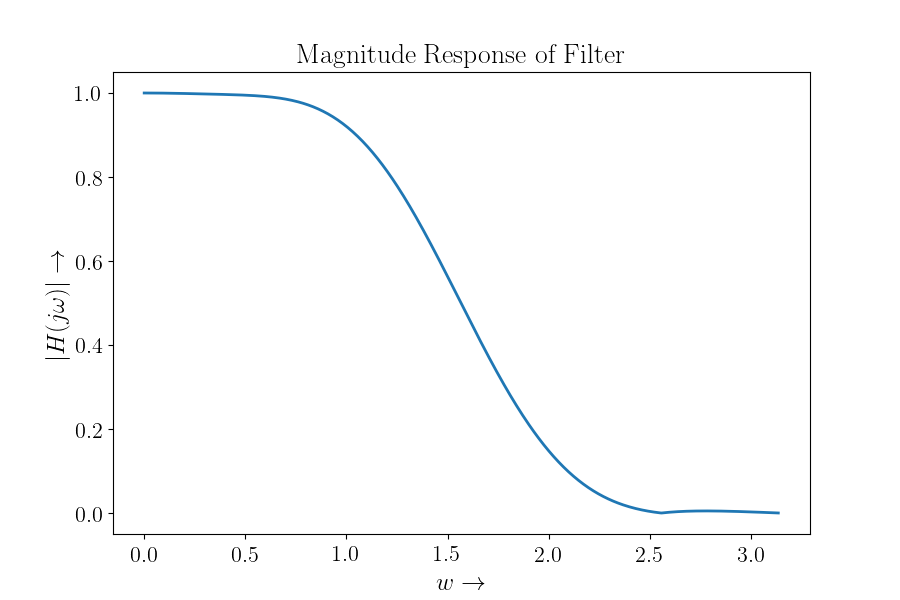
\includegraphics[scale=0.6]{./../Extras/a10-1.png}  % Mention the image name within the curly braces. Image should be in the same folder as the tex file.  
  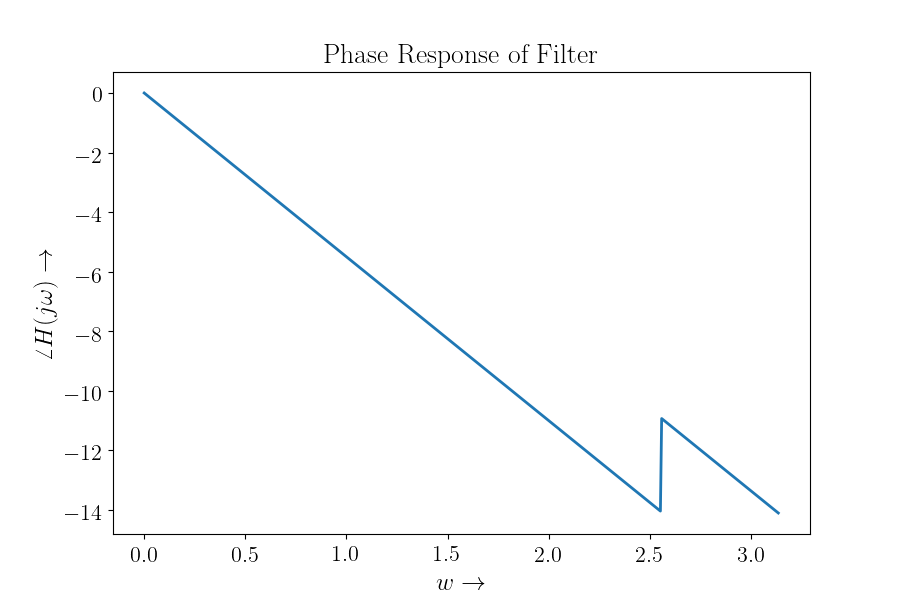
\includegraphics[scale=0.6]{./../Extras/a10-2.png}  % Mention the image name within the curly braces. Image should be in the same folder as the tex file.  
  \caption{Magnitude and Phase Response of Filter}
\end{figure}
\newpage
\subsubsection{Results \& Discussion:}\label{results-discussion}
\begin{itemize}
  \item From the phase plot, we can see that the filter is a $Lowpass$ $Filter$. The 3db cutoff frequency is approximately $30^{o}$.
  \item From the phase plot, we can conclude that the given filter is a $Linear$ $Fitler$. Thus, there will be a time delay in the output of the function while compared to the input function
\end{itemize}
\newpage
\subsection{Question 2}
\begin{itemize}
  \item Generate the function $x[n] = cos(0.2\pi n)+cos(0.85\pi n) $ for $n \in [0,1024]$.
  \item Pass it through the filter via linear convolution and circular convolution. Observe the differences
\end{itemize}
\textit{\textbf{Code:}}

\begin{lstlisting}
n = np.linspace(0, 1024, 1025)
n = n[:-1]
x = np.cos(np.pi*0.2*n)+np.cos(0.85*np.pi*n)

plt.title(r"$x[n] = cos(0.2\pi n)+cos(0.85\pi n)$")
plt.stem(n, x)
plt.xlabel(r"$n \to$")
plt.ylabel(r"$x[n] \to$")
plt.show()

plt.title(r"$x[n]$ for n $\in$ [0,100]")
plt.stem(n, x)
plt.xlabel(r"$n \to$")
plt.ylabel(r"$x[n] \to$")
plt.xlim([0, 100])
plt.show()

\end{lstlisting}
\newpage
\begin{figure}[!tbh]
  \centering
  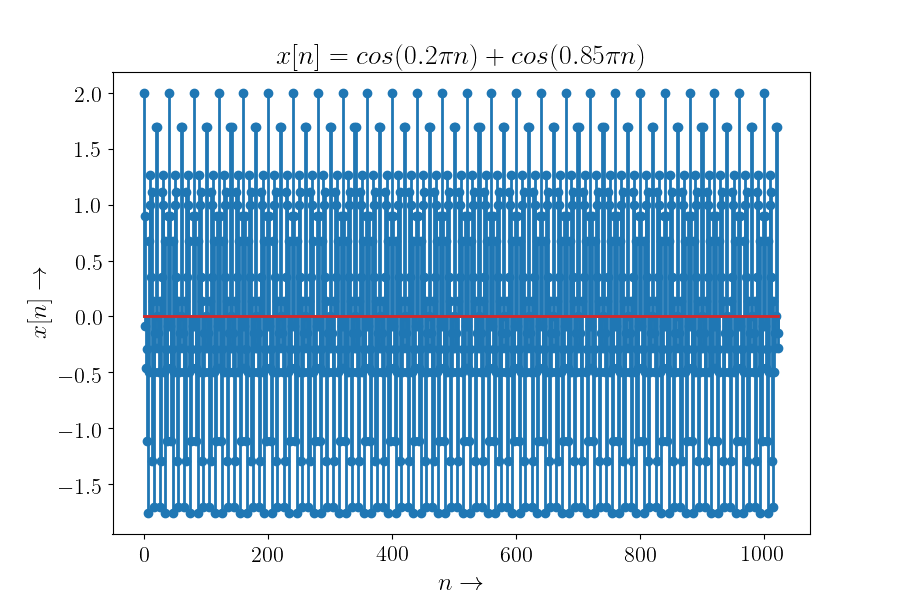
\includegraphics[scale=0.6]{./../Extras/a10-3.png}  % Mention the image name within the curly braces. Image should be in the same folder as the tex file.  
  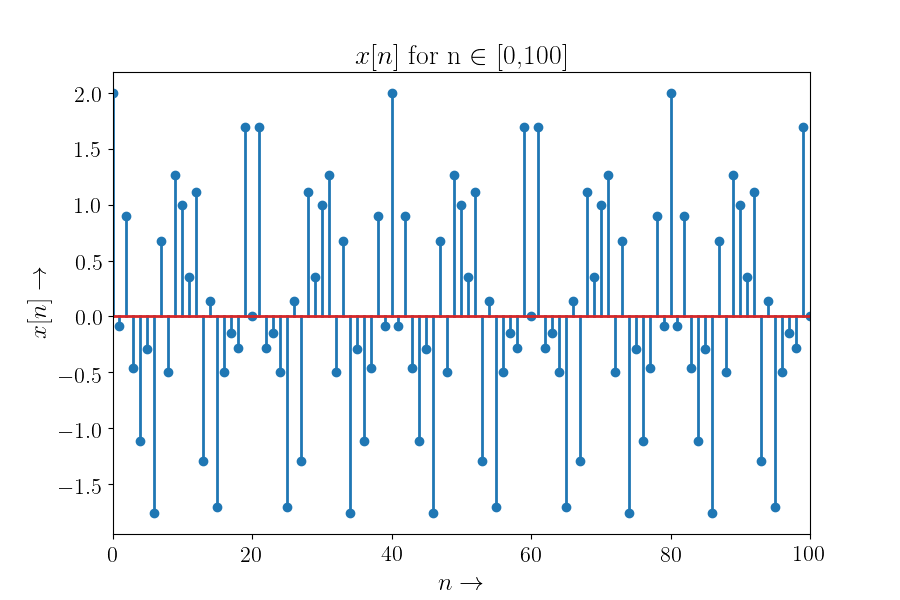
\includegraphics[scale=0.6]{./../Extras/a10-4.png}  % Mention the image name within the curly braces. Image should be in the same folder as the tex file.  
  \caption{$x[n] = cos(0.2\pi n)+cos(0.85\pi n) $}
\end{figure}
\newpage
\textit{\textbf{Code:}}
\begin{lstlisting}
y_conv = np.convolve(x, fil)

plt.title(r"$y[n] = x[n]*h[n]$")
plt.stem(y_conv)
plt.xlabel(r"$n \to$")
plt.ylabel(r"$y[n] \to$")
plt.show()

plt.xlim([0, 100])
plt.title(r"$y[n]$ zoomed to start")
plt.stem(y_conv)
plt.xlabel(r"$n \to$")
plt.ylabel(r"$y[n] \to$")
plt.show()


plt.xlim([900, 1050])
plt.title(r"$y[n]$ zoomed to end")
plt.stem(y_conv)
plt.xlabel(r"$n \to$")
plt.ylabel(r"$y[n] \to$")
plt.show()

fil_rep = np.concatenate([fil, np.zeros(len(x) - len(fil))])
y1 = np.fft.ifft(np.fft.fft(x)*np.fft.fft(fil_rep))


plt.title(r"$y'[n] = x[n] \circledast h[n]$")
plt.stem(y1)
plt.xlabel(r"$n \to$")
plt.ylabel(r"$y'[n] \to$")
plt.show()

plt.xlim([0, 100])
plt.title(r"$y'[n]$ zoomed to start")
plt.stem(y1)
plt.xlabel(r"$n \to$")
plt.ylabel(r"$y'[n] \to$")
plt.show()


plt.xlim([900, 1050])
plt.title(r"$y'[n]$ zoomed to end")
plt.stem(y1)
plt.xlabel(r"$n \to$")
plt.ylabel(r"$y'[n] \to$")
plt.show()
  \end{lstlisting}
\newpage
\begin{figure}[!tbh]
  \centering
  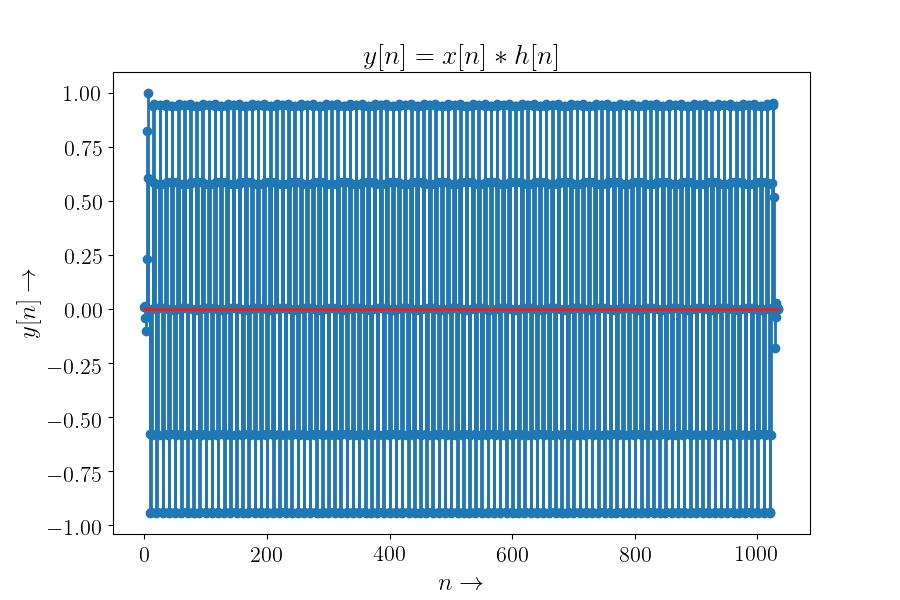
\includegraphics[scale=0.4]{./../Extras/a10-5.png}  % Mention the image name within the curly braces. Image should be in the same folder as the tex file.  
  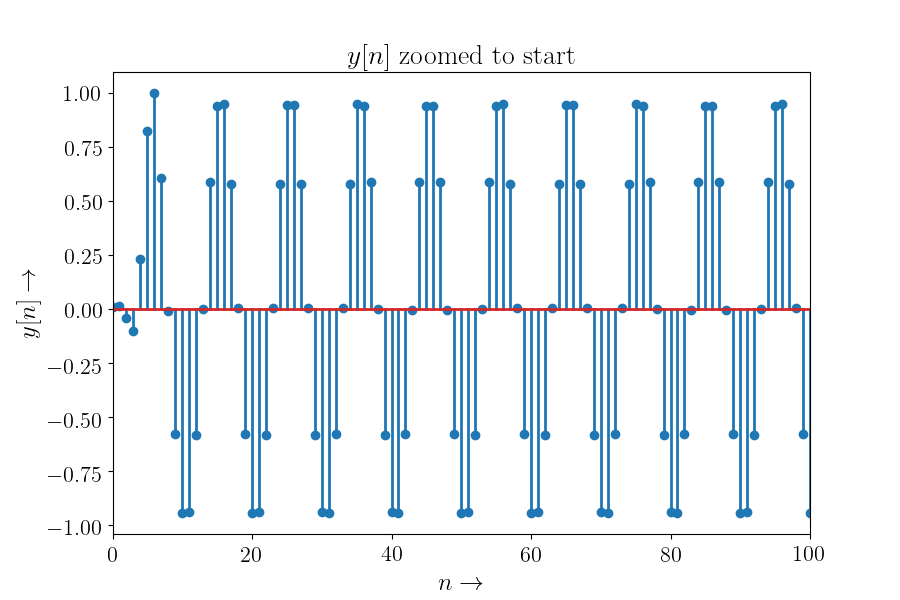
\includegraphics[scale=0.4]{./../Extras/a10-6.png}  % Mention the image name within the curly braces. Image should be in the same folder as the tex file.  
  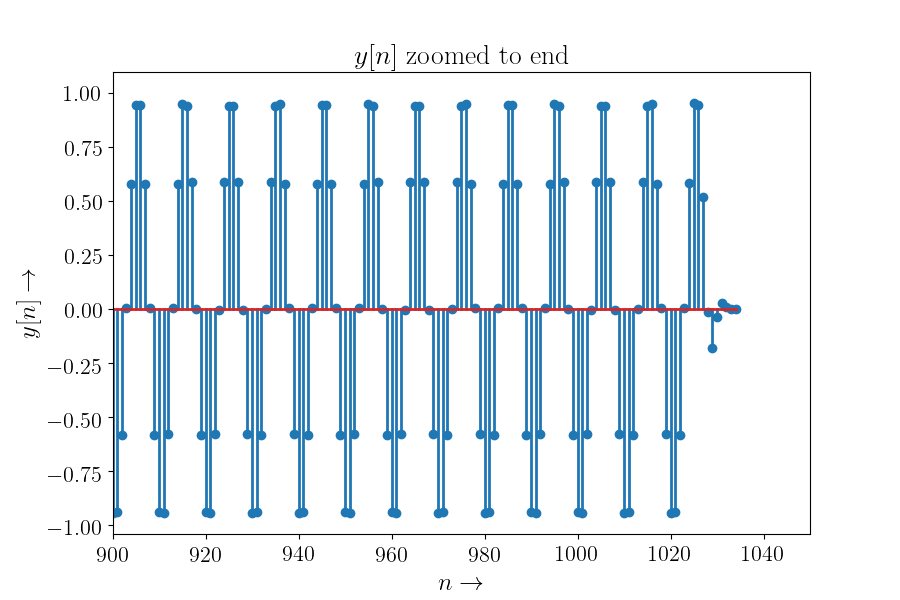
\includegraphics[scale=0.4]{./../Extras/a10-7.png}  % Mention the image name within the curly braces. Image should be in the same folder as the tex file.  
  \caption{Linear Convolution}
\end{figure}
\newpage
\begin{figure}[!tbh]
  \centering
  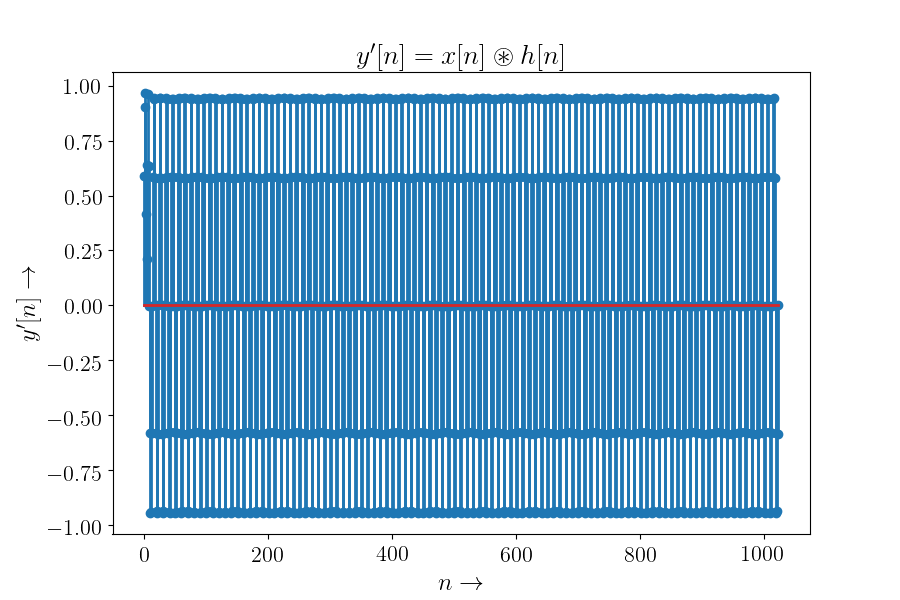
\includegraphics[scale=0.4]{./../Extras/a10-8.png}  % Mention the image name within the curly braces. Image should be in the same folder as the tex file.  
  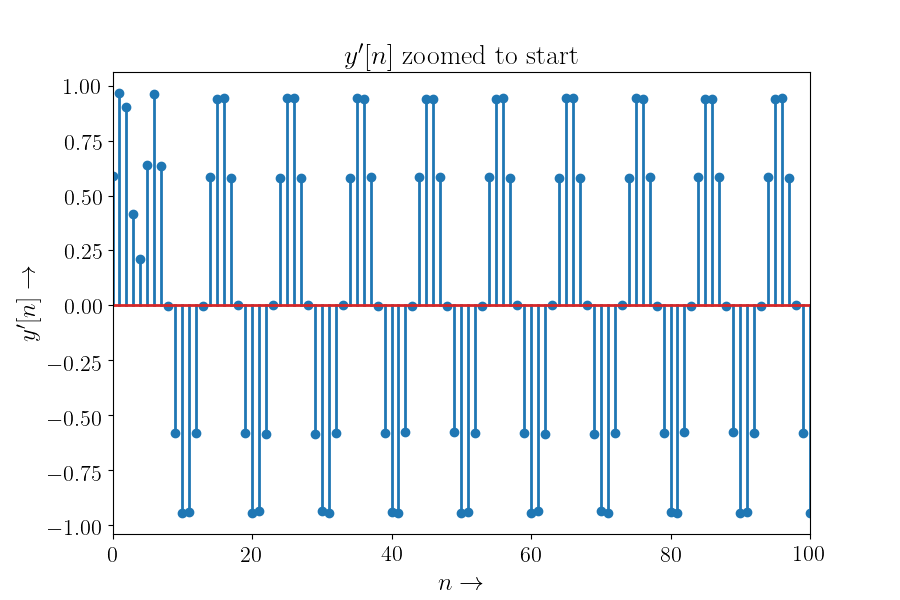
\includegraphics[scale=0.4]{./../Extras/a10-9.png}  % Mention the image name within the curly braces. Image should be in the same folder as the tex file.  
  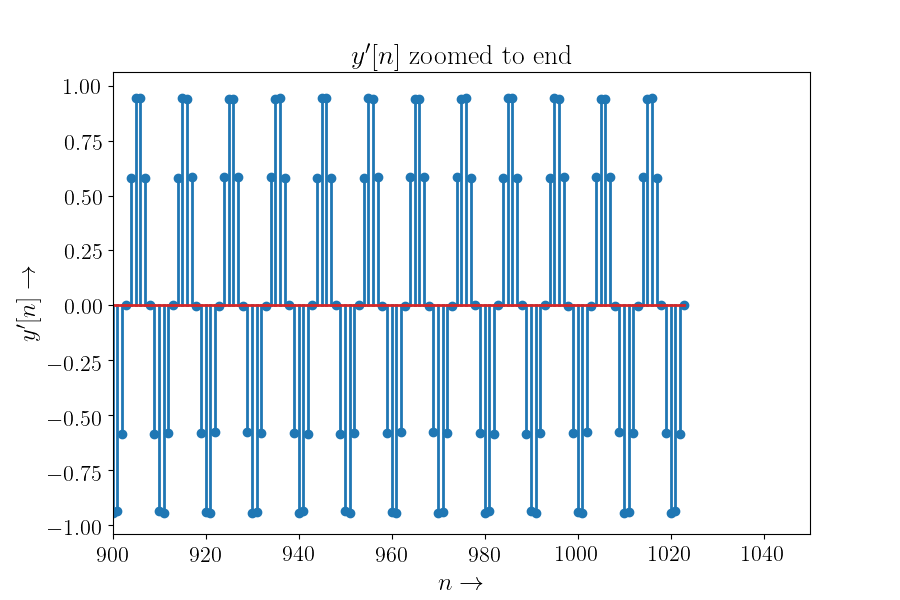
\includegraphics[scale=0.4]{./../Extras/a10-10.png}  % Mention the image name within the curly braces. Image should be in the same folder as the tex file.  
  \caption{Circular Convolution}
\end{figure}
\newpage
\subsubsection{Results \& Discussion:}\label{results-discussion}
\begin{itemize}
  \item There are distinct differences in both the convolutions
  \item One of the main difference is that the output of both the convolutions are not of same size.
  \item Also in the start, both the convolutions do not look similar, although they do so afterwards.
  \item This is expected behaviour, since the method by which we find the convolutions differ greatly and this is reflected in their output
\end{itemize}
\newpage
\subsection{Question 3}
\begin{itemize}
  \item Now we are to convolve both the signals linearly using circular convolution
\end{itemize}
\textit{\textbf{Code:}}
\begin{lstlisting}
x_split = np.array(np.split(x, 1024/16))
P = len(fil)
L = x_split.shape[1]
N = L+P-1
y_part = np.zeros((x_split.shape[0], N))
fil_new = np.concatenate([fil, np.zeros(N-len(fil))])
for i in range(x_split.shape[0]):
    x_new = np.concatenate([x_split[i], np.zeros(N-len(x_split[i]))])
    y_part[i] = np.array(np.fft.ifft(np.fft.fft(x_new)*np.fft.fft(fil_new)))
y = np.zeros(len(x)+len(fil))

J = len(y_part[0])
K = J-(P-1)
for i in range(y_part.shape[0]):
    y[i*K:i*K+J] += y_part[i]


plt.title(r"$y[n] = x[n]*h[n]$ using circular convolution")
plt.stem(y)
plt.xlabel(r"$n \to$")
plt.ylabel(r"$y'[n] \to$")
plt.show()
\end{lstlisting}
\newpage
\begin{figure}[!tbh]
  \centering
  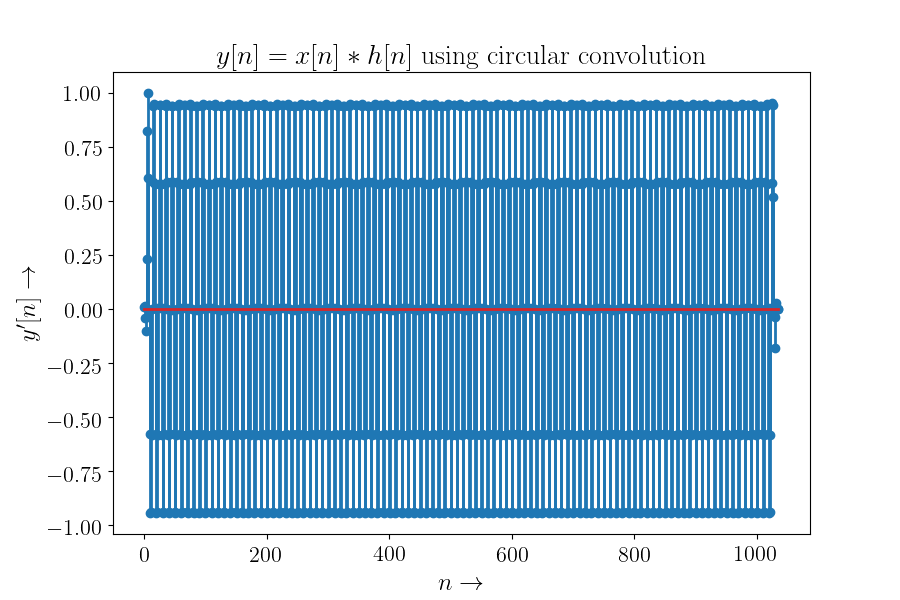
\includegraphics[scale=0.6]{./../Extras/a10-11.png}  % Mention the image name within the curly braces. Image should be in the same folder as the tex file.  
  \caption{Linear Convolution using Circular Convolution}
\end{figure}
\newpage
\subsubsection{Results \& Discussion:}\label{results-discussion}
\begin{itemize}
  \item Thus, we have done the linear convolution using circular convolution
\end{itemize}
\newpage

\subsection{Question 4}
\begin{itemize}
  \item We are going to analyse the Zadoff-Chu by both linearly autocorrelating and circularly autocorrelating it with a cyclic shifted version of the signal
  \item Correlation is given by 
\end{itemize}
  \begin{equation}
   y[n] = x[n]*h[-n]
  \end{equation}
  \begin{itemize}
  \item Autocorrelation is when a signal is correlated with itself
  \item The definition holds in circular correlation too, i.e.
  
  \begin{equation}
    y[n] = x[n]\circledast h[-n]
   \end{equation}
   \item In DFT domain, it becomes
   \begin{equation}
    Y[m] = X[m]H^{*}[m]
   \end{equation}
   \item $H^{*}[m]$ is the conjugate of $H[m]$
\end{itemize}
\textit{\textbf{Code:}}
\begin{lstlisting}
z_c = pd.read_csv("/home/omshripc/Sem 4/EE2703/Answers/x1.csv",
                  header=None).values[:, 0]

z_c = np.array([complex(z_c[i].replace("i", "j")) for i in range(len(z_c))])


plt.title(r"Magnitude of Zadoff-Chu sequence ($z[n]$)")
plt.plot(np.round(np.abs(z_c)), 'bo')

plt.xlabel(r"$n \to$")
plt.ylabel(r"$z[n] \to$")
plt.show()

z_c_rot = np.concatenate([z_c[5:], z_c[0:5]])

y_corr = np.correlate(z_c, z_c_rot, "full")
n = np.linspace(-len(z_c), len(z_c), len(y_corr))

plt.title(r"$p[n]$ = Correlation of $z[n]$ with z[n] cyclically shifted by n=5")

plt.stem(n, np.abs(y_corr))
plt.xlabel(r"$n \to$")
plt.ylabel(r"$p[n] \to$")
plt.show()

plt.title(r"$p[n]$ for n $\in$ [3,7]")
plt.stem(n, np.abs(y_corr))
plt.xlim([3, 7])
plt.xlabel(r"$n \to$")
plt.ylabel(r"$p[n] \to$")
plt.show()

y_cir_conv = np.fft.ifft(np.fft.fft(z_c)*np.fft.fft(np.conj(z_c_rot)))
plt.title(
    r"$q[n]$ = Circular Correlation of $z[n]$ with z[n] cyclically shifted by n=5")

plt.stem(np.abs(y_cir_conv))
plt.xlabel(r"$n \to$")
plt.ylabel(r"$p[n] \to$")
plt.show()

plt.title(r"$q[n]$ for n $\in$ [830,838]")
plt.stem(np.abs(y_cir_conv))
plt.xlim([830, 838])
plt.xlabel(r"$n \to$")
plt.ylabel(r"$p[n] \to$")
plt.show()
\end{lstlisting}
\newpage
\begin{figure}[!tbh]
  \centering
  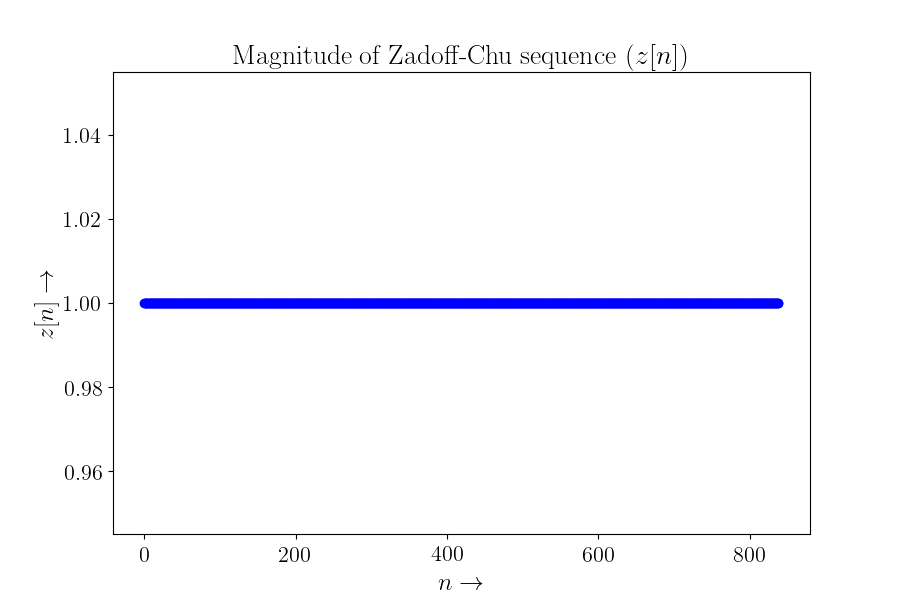
\includegraphics[scale=0.6]{./../Extras/a10-12.png}  
  \caption{Magnitude of Zandoff-Chu sequence}
\end{figure}
\newpage
\begin{figure}[!tbh]
  \centering
  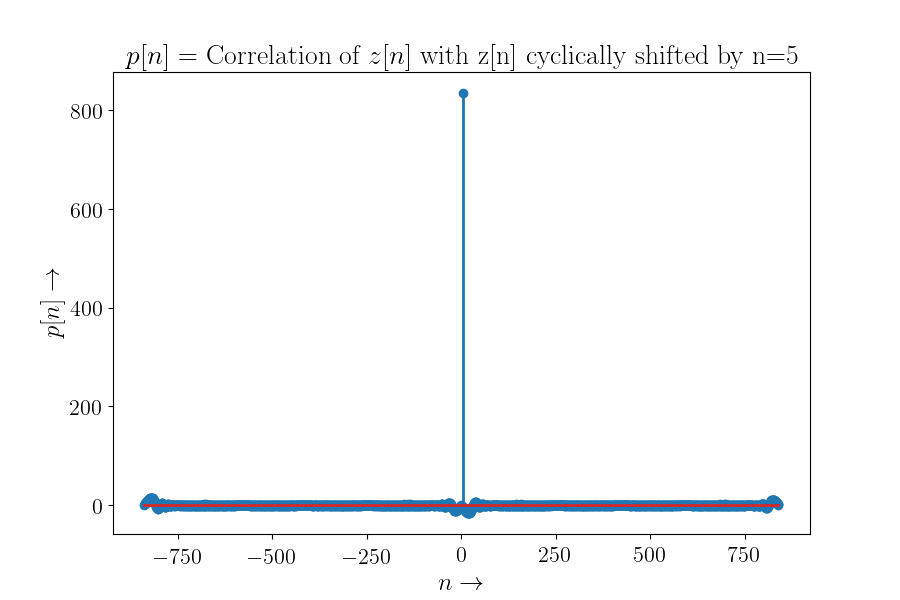
\includegraphics[scale=0.6]{./../Extras/a10-13.png}  
  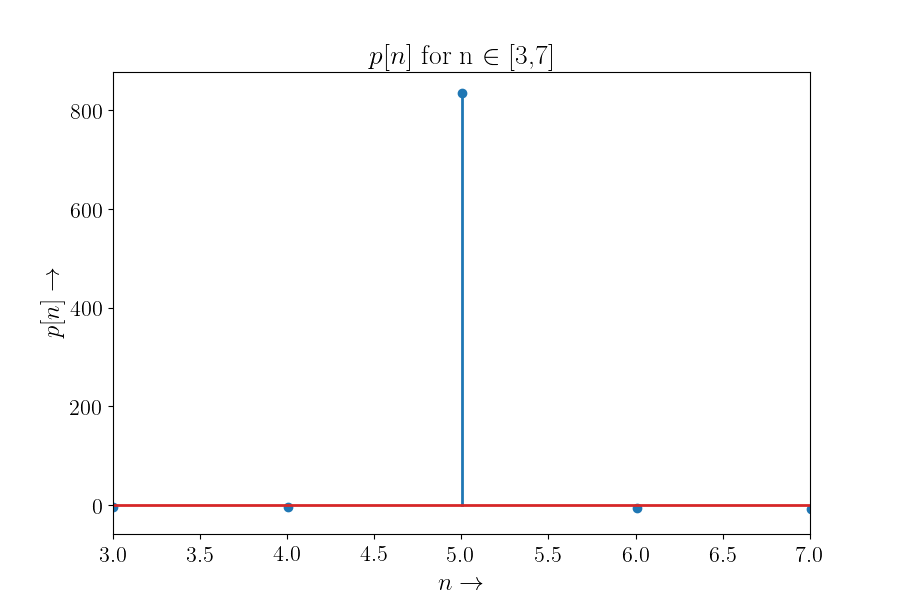
\includegraphics[scale=0.6]{./../Extras/a10-14.png}  
  \caption{Linear Convolution of Zandoff-Chu sequence}
\end{figure}
\newpage
\begin{figure}[!tbh]
  \centering
  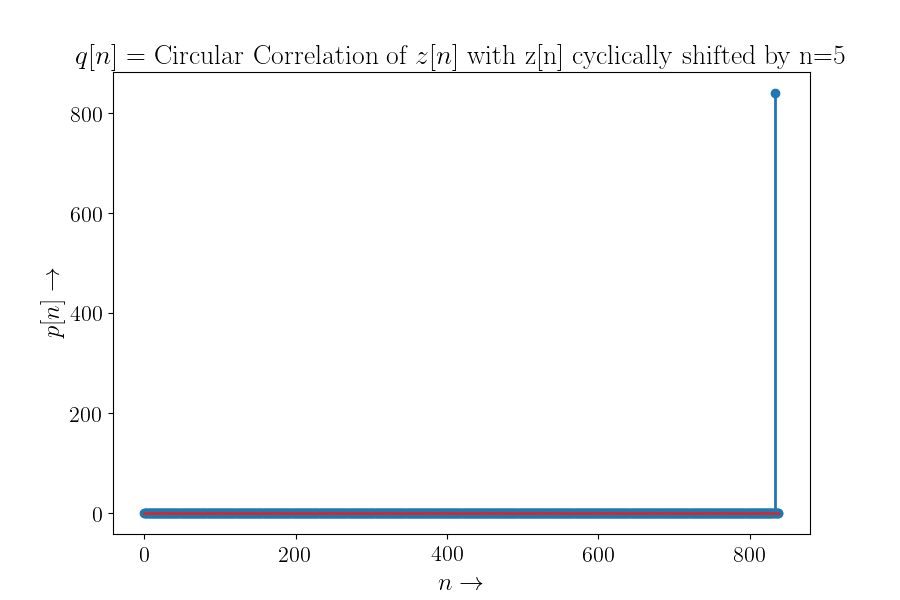
\includegraphics[scale=0.6]{./../Extras/a10-15.png}  
  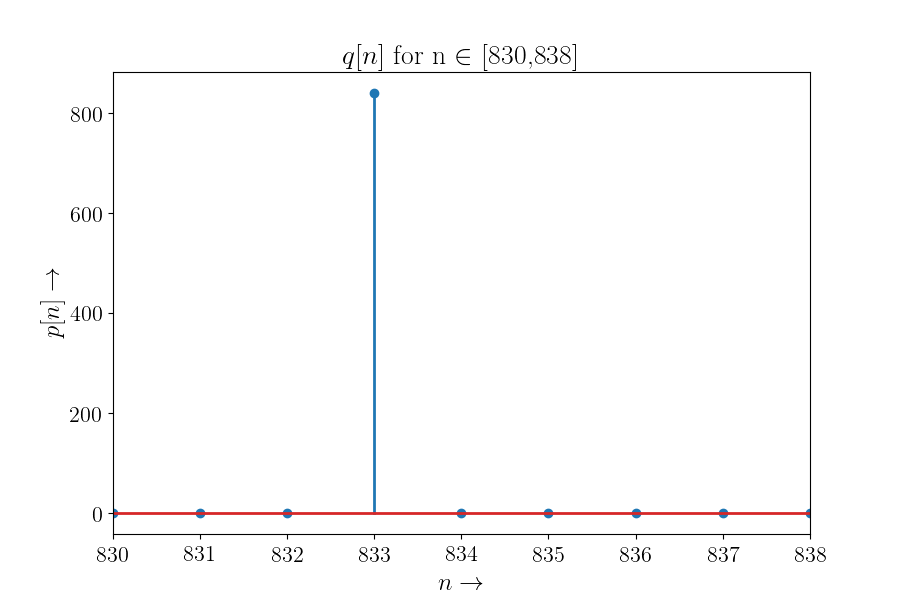
\includegraphics[scale=0.6]{./../Extras/a10-16.png}  
  \caption{Linear Convolution of Zandoff-Chu sequence}
\end{figure}
\newpage
\subsubsection{Results \& Discussion:}\label{results-discussion}
\begin{itemize}
  \item We see that the magnitude of the Zandoff-Chu sequence is 1, which is a property of the sequence
  \item We can clearly see that there are peaks at the particular points and the function is zero at all other points
  \item The peak is at the value by which we cyclically shifted our signal for the linear convolution, but it is peaking at the value of shift from the last for the circular correlation
  \item This is the special property of the Zandoff-Chu sequence, i.e. the correlation of the sequence with a cyclic shifted version of it is zero everywhere but only peaks at the value of its shift.
  \item Also, since the circular correlation is defined as such,  the peak now occurs at the value of shift from the last.
\end{itemize}
\section{Conclusion}
  Thus we were able to linearly convolve two signals using circular convolution and were also able to study the property of Zandoff-Chu sequence

\end{document}